\documentclass{article}
\pdfoutput=1
\usepackage{tikz}
\usetikzlibrary{arrows,automata,backgrounds,calc,chains,fadings,folding,decorations.fractals,decorations.pathreplacing,fit,patterns,positioning,mindmap,shadows,shapes.geometric,shapes.symbols,through,trees,plotmarks}

\newcommand{\charlie}{\texttt{Charlie}}
\newcommand{\cora}{\texttt{Cora}}

\begin{document}

\section*{The overall structure and dependencies of Charlie}

The picture below illustrates the package dependencies in \charlie: the core constrained
higher-order rewriting library used in \cora.  Note that there are no mutual dependencies:
every package only depends on those packages above it that it is connected to; that is, A depends
on B if there is a path from B to A following the arrow directions.  For example,
\texttt{charlie.parser} may use classes from \texttt{charlie.exceptions}, \texttt{charlie.util},
\texttt{charlie.parser.lib} and \texttt{charlie.types}, but not from (e.g.) \texttt{charlie.smt} or
\texttt{charlie.reader}.

\begin{center}
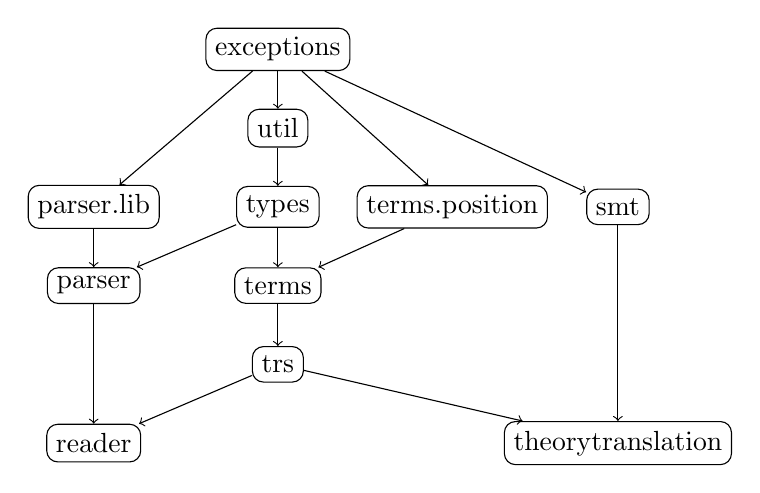
\begin{tikzpicture}[->]
\tikzstyle{veld} = [draw, fill=white, minimum height=0em, minimum width=0em, rounded corners]

\node [veld] (exceptions) {exceptions};
\node [veld] (util) [below of=exceptions, node distance=10mm] {util};
\draw (exceptions) -- (util);

\node [veld] (types) [below of=util, node distance=10mm] {types};
\draw (util) -- (types);

\node [veld] (parserlib) [left of=types, node distance=15mm, anchor=east] {parser.lib};
\draw (exceptions) -- (parserlib);

\node [veld] (parser) [below of=parserlib, node distance=10mm] {parser};
\draw (parserlib) -- (parser);
\draw (types) -- (parser);

\node [veld] (termspos) [right of=types, node distance=10mm, anchor=west] {terms.position};
\draw (exceptions) -- (termspos);

\node [veld] (smt) [right of=termspos, node distance=17mm, anchor=west] {smt};
\draw (exceptions) -- (smt);

\node [veld] (terms) [below of=types, node distance=10mm] {terms};
\draw (types) -- (terms);
\draw (termspos) -- (terms);

\node [veld] (trs) [below of=terms, node distance=10mm] {trs};
\draw (terms) -- (trs);

\node [veld] (reader) [below of=parser, node distance=20mm] {reader};
\draw (parser) -- (reader);
\draw (trs) -- (reader);

\node [veld] (theory) [below of=smt, node distance=30mm] {theorytranslation};
\draw (trs) -- (theory);
\draw (smt) -- (theory);

\end{tikzpicture}
\end{center}

\end{document}

